\documentclass{llncs}

\usepackage{cite}
\usepackage{amsmath,amssymb}
\usepackage{graphicx}
\usepackage{booktabs}
\usepackage{multirow}
\usepackage{array}
\usepackage{url}
\usepackage{float}
\usepackage{fancyhdr}
\usepackage[skip=2pt]{caption}
\usepackage{placeins}
\usepackage{etoolbox}
\linespread{0.95}

% ----------- FIX SPACING ISSUES -----------
\setlength{\textfloatsep}{4pt}
\setlength{\floatsep}{4pt}
\setlength{\intextsep}{4pt}

\pagestyle{fancy}
\fancyhf{}
\fancyhead[L]{\small Federated Learning for Massive MIMO Channel Estimation}
\fancyhead[R]{\small\thepage}
\renewcommand{\headrulewidth}{0.4pt}

\title{Federated Learning for Massive MIMO Channel Estimation Under IID and Non-IID Client Data}

\author{Jagadeesh Kakarla \and Koppaku Krishna Chaitanya \and Kappala Akshay \and Dammala Basava Sri ram \and Yaparla Sainatha reddy}
\institute{Indian Institute of Information Technology, Design and Manufacturing, Kancheepuram\\
\email{jagadeeshk@iiitdm.ac.in, krish23306@gmail.com, dammala.sriram9@gmail.com, akshaykappala1029@gmail.com, sainathreddy057@gmail.com}}

\begin{document}

\maketitle

\begin{abstract}
Channel estimation in wireless communication recently became capable of harnessing the power of deep learning techniques. However, conventional techniques for channel estimation rely on the centralized setting, which suffers from high
communication costs and privacy issues. To address these issues, in this paper, we present a federated learning approach
for channel estimation in massive MIMO systems. The proposed
approach involves training convolutional and encoder-decoder
(ResUNet) architectures via FedAvg and FedProx on IIDs and
non-IIDs clients, respectively. Our reproducibly available benchmark confirms that our federated approach provides good estimation results and, in particular, outperforms the centralized counterpart when FedAvg is run in IID setting by only 0.32 dB (-20.04 dB vs. -19.62 dB NMSE). In addition, we analyze the effect of non-IIDs on channel estimation and show that there is up to a 0.3 dB accuracy gap that can be mitigated via FedProx.
\keywords{Federated learning \and massive MIMO \and channel estimation \and non-IID data \and FedAvg \and FedProx \and reproducibility}
\end{abstract}

\section{Introduction}
The development of wireless communications to 5G and further to 6G requires the achievement of very high spectral efficiency, massive connectivity, and ultra-reliable low-latency communications. In order to fulfill these challenging needs, the
architecture of Massive Multiple Input Multiple Output (Massive MIMO) system is proposed. With many antennas on the base station (BS) side, Massive MIMO uses spatial multiplexing and directional beamforming to support multiple users through the same frequency-time resources at the same time.

Nonetheless, for the realization of the advantages of Massive MIMO, accurate information about the Channel State Information (CSI) at the BS becomes critical. It is here that the estimation of the channel becomes critical since the objective involves the estimation of the channel environment between the transmit antenna and the receive antenna using pilot signals. In the case of massive MIMO, the complexity in calculating the CSI arises from the fact that there are many dimensions within the channel matrix. The techniques commonly used for linear estimation include LS and MMSE.

In order to address the shortcomings associated with classic heuristics, the latest developments within Deep Learning (DL) have shown tremendous success in estimating massive MIMO channel ~\cite{wen2018deep, he2018deep, ye2018power, soltani2019deep}. The DL algorithm learns to implicitly
map the complex, non-linear relationships in the wireless channel and avoids the need for costly inversions of high-dimensional matrices. However, traditional DL techniques require a centralized approach to learning. Under such an approach, the user equipment (UE) would be required to continually send its highly dimensional local pilots/CSI measurements to the central server for training the model.Centralized learning results in heavy communication overheads and serious privacy issues.

This is where Federated Learning (FL) emerges as an interesting option as it allows training of a globally good model by means of locally updating the system without the need for any transfer of the channel information at all~\cite{kairouz2021survey, ghosh2019robust}. However, although FL already addresses issues like privacy and minimization of uplink payload by its very nature, performance becomes sensitive to client heterogeneity when UE datasets become Non-IID because of geographical diversity and signal-to-noise ratio (SNR)  values.

In this paper, we attempt to conduct an exhaustive analysis for channel estimation in FL based on both IID and Non-IID scenarios. The performances of FedAvg and the Proximal Regularization technique called FedProx have been compared using both light weight CNN architecture and heavy ResUNet architecture.

\subsection{Contributions}
\begin{itemize}
    \item Channel estimation using raw-to-paper reproducibility traceability, IID/Non IID evaluation for FedAvg and FedProx, cross architecture validation using CNN and ResUNet, and communication-runtime-model size evaluation for realistic applications.
\end{itemize}

\section{Related Work}
The closest related work to this research can be found in Elbir and Coleri ~\cite{elbir2021flchannel}. We have similar objectives of achieving channel estimation via FL and minimizing overhead through communication. The protocols used are not identical, so we present this as partially matching.


Elbir and Coleri provide a definite framework in which CL involves the transfer of user data sets to the BS, whereas FL involves only the transmission of model update information, reducing the cost of communication without compromising estimation performance compared to CL ~\cite{elbir2021flchannel}. We follow this framework in our manuscript organization and present pipeline-level trade-offs instead of endpoint NMSE values.

In concrete terms, their approach involves: (i) estimation of FL channel in conventional as well as RIS-enabled massive MIMO; (ii) overhead analysis relative to CL; and (iii) robustness analysis for noisy/quantized/lossy model updates.
They report that their method results in an overhead reduction factor of approximately 16 compared to CL in their framework. For further background on machine learning and federated approaches in current wireless networks, including RIS, refer to the comprehensive survey paper by Faisal and Choi~\cite{faisal2022rismlsurvey}. Founda-
tional papers in the field of federated learning are FedAvg~\cite{mcmahan2017fedavg} and FedProx~\cite{li2020fedprox}.


For comparison purposes,  Table~\ref{tab:alignment_ec} lists what is directly comparable to
Elbir–Coleri ~\cite{elbir2021flchannel} and what is comparable based on context.

\begin{table}[htbp]
\caption{Detailed Alignment With Elbir--Coleri~\cite{elbir2021flchannel}}
\label{tab:alignment_ec}
\centering
\begin{tabular}{p{0.25\linewidth}p{0.34\linewidth}p{0.30\linewidth}}
\toprule
Aspect & Elbir--Coleri (TWC) & This Work \\
\midrule
Primary motivation & Reduce CL data-transfer overhead via FL & Same motivation and FL framing \\
Task & FL channel estimation & FL channel estimation \\
Scenarios & Conventional + RIS-assisted massive MIMO & Massive MIMO benchmark (DeepMIMO O1\_60) \\
Model family & CNN-based ChannelNet & CNN (primary) + ResUNet (add-on) \\
Learning modes & CL vs FL & CL vs FL (FedAvg/FedProx) \\
Heterogeneity \\ analysis & Non-i.i.d. challenge discussed & Explicit IID/Non-IID protocol and quantified deltas \\
Update-channel \\ robustness & Noisy, quantized, partial-loss model updates & Communication/runtime analysis; update-channel robustness left for future extension \\
Overhead reporting & Reports \textasciitilde16$\times$ lower overhead vs CL & Communication events + payload model (4PKR) \\
Comparison level & Domain reference benchmark & Partial-match external comparison \\
\bottomrule
\end{tabular}
\end{table}



\section{System Model and Problem Formulation}

\begin{figure}[htbp]
\centering
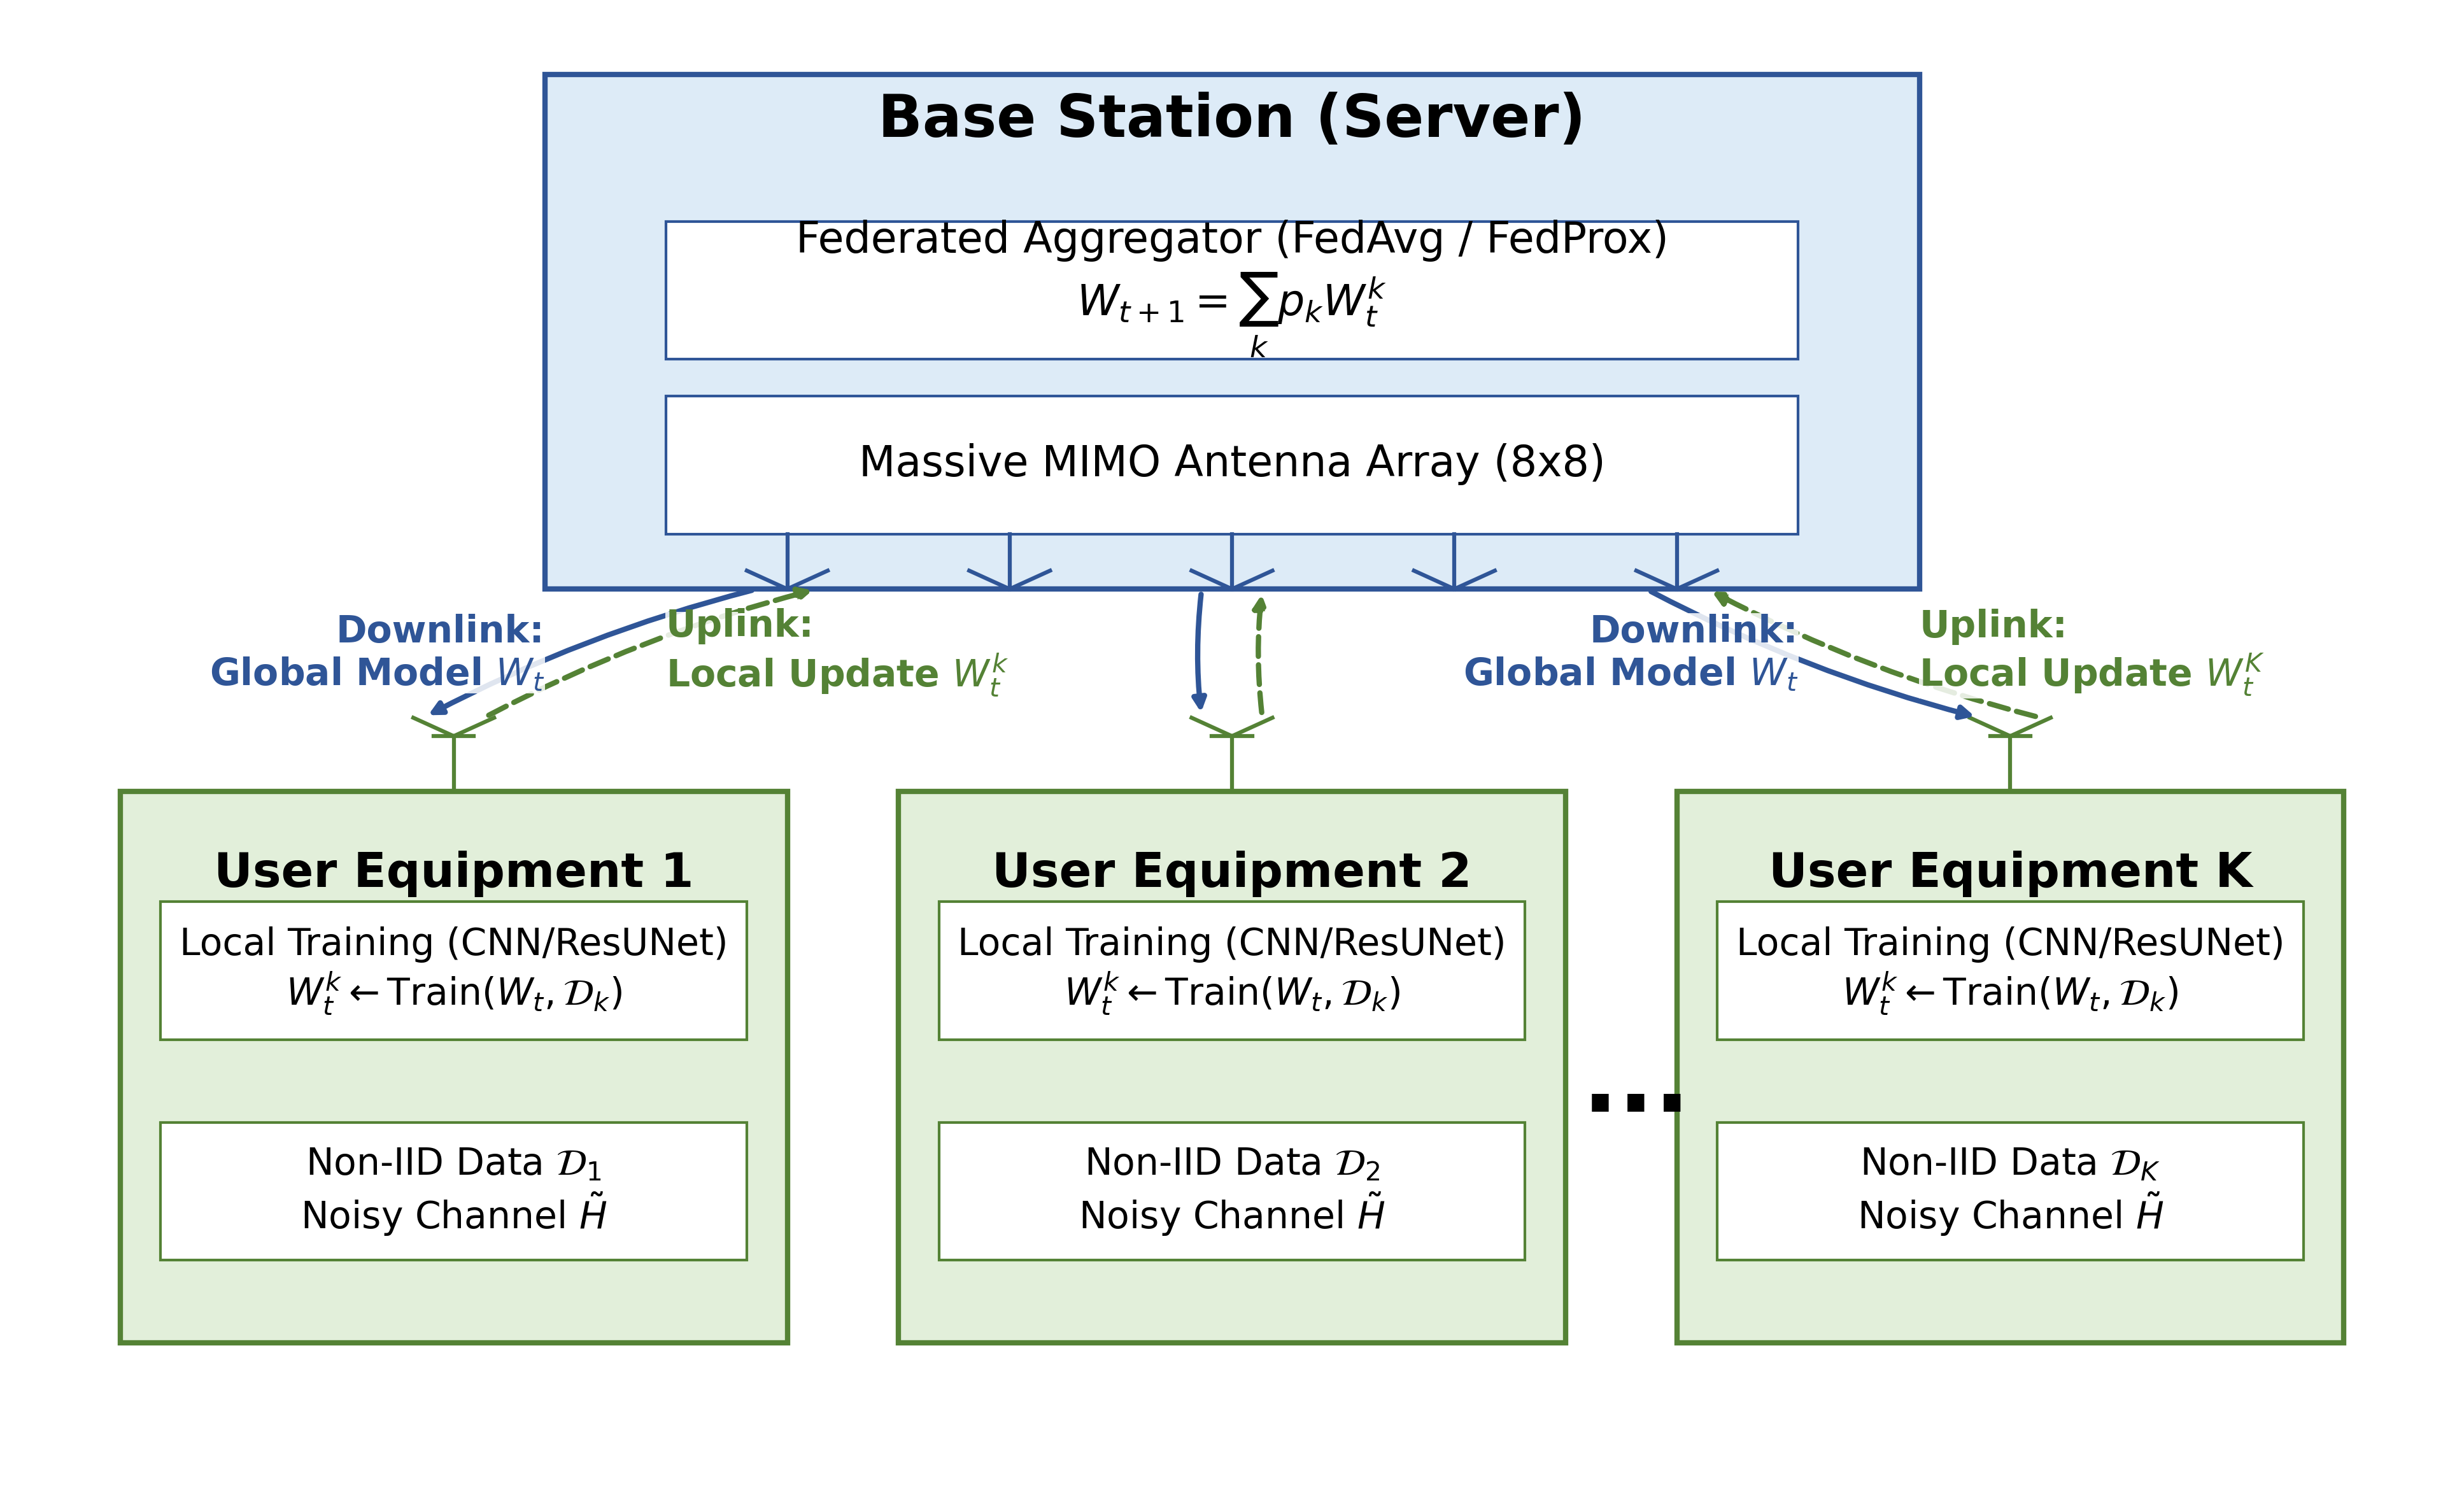
\includegraphics[width=\columnwidth]{figures/system_architecture_diagram.png}
\caption{Architecture diagram of the Massive MIMO Federated Learning system. The Base Station acts as the server, where it aggregates the model updates from multiple User Equipments (clients) without requiring raw channel data transmission.}
\label{fig:system_model}
\end{figure}


Let $H\in\mathbb{C}^{N_t\times N_s}$ denote the clean channel response and $\tilde H$ the noisy observation from pilot-based acquisition. The estimator outputs $\hat H=f_\theta(\tilde H)$. Performance is measured by normalized mean squared error (NMSE):
\begin{equation}
\mathrm{NMSE}_{\mathrm{dB}} = 10\log_{10}\left(\frac{\|H-\hat{H}\|_2^2}{\|H\|_2^2}\right).
\end{equation}

In CL, all training samples are centrally aggregated. In FL, each client $k$ trains locally and sends model updates to server. FedAvg aggregation is:
\begin{equation}
\theta^{t+1} = \sum_{k=1}^{K} \frac{n_k}{\sum_j n_j}\theta_k^t,
\end{equation}
where $n_k$ is local dataset size. FedProx solves per-client local objective:
\begin{equation}
\min_{\theta_k} F_k(\theta_k) + \frac{\mu}{2}\|\theta_k-\theta^t\|_2^2.
\end{equation}

\section{Proposed Methodology}
This proposed methodology would follow the below pipeline which consists of six stages, namely; (i) channel generation using the DeepMIMO ray tracing simulator, (ii) adding AWGN noise at varying SNR values, where power normalization is done for each sample, (iii) global data normalization and data set split for train and test data set, (iv) client data distribution following IID and Non-IID distribution, (v) Federated learning-based model training using FedAvg and FedProx algorithms, where two different CNN and ResUnet based architectures will be trained, and (vi) evaluation of models' performance through the NMSE metric using the holdout test data set. Model training will be carried out locally using all clients through the Adam optimizer to minimize the MSE cost function.

\subsection{Dataset Construction}
The dataset is derived from DeepMIMO O1\_60. We select 6000 users from BS-0, configure an 8$\times$8 BS array, 1$\times$1 UE array, and 64 OFDM subcarriers. The AWGN noise is added to the SNR of \{0,5,10,15,20\} dB after sample-wise normalization using the same random number generator seed (42). Real/imaginary channel data are saved as well.

In the case of supervised learning, the samples and labels are normalized, randomly shuffled, and then split for training and testing in an 80/20 ratio per each SNR level.

\subsection{Models}
\textbf{CNN (Primary Benchmark):} A light-weight residual convolutional neural network architecture that learns the residual correction to noise ($\Delta H = H_{\text{noisy}} - H_{\text{clean}}$) as opposed to learning a mapping of the entire channel. The model comprises a feature extraction head (a 2D Convolutional layer that maps from 2 to 32 channels,
followed by BatchNorm and ReLU), a residual body composed of a single \texttt{ResidualBlock} (2x 32-channel Convolutions with skip connection), and a reconstruction tail (2D Convolution from 32 channels back to 2 channels). The model is very efficient, using only 19,778 trainable parameters.




\textbf{ResUNet (Cross-Architecture Validation):} A larger capacity and multi-scale encoder-decoder network model (763,234 parameters) used to verify that our findings about
FL heterogeneity generalize beyond light-weight models. The architecture comprises 15 layers. The architecture has an encoder side comprising three ConvBlock sequences, which reduce the spatial dimensions of the signal while increasing its channel capacity (from 2 to 128 channels), a residual bottleneck, and a decoder side which upsamples the signal using Transpose Convolutions. The decoder side uses skip connections to concatenate features extracted on high resolution by the encoder side with the upsampled features.

\subsection{IID and Non-IID Definitions}
IID partitions are generated by global shuffle and uniform client split.

For Non-IID, we use reproducible client-level distribution skew. In ResUNet FL, client dataset is explicitly formed as
\begin{equation}
\mathcal{D}_k=\mathcal{D}_k^u \cup \mathcal{D}_k^s,\quad \rho=\frac{|\mathcal{D}_k^u|}{|\mathcal{D}_k|},
\end{equation}
with $\rho=0.6$ unique norm-sorted segment and 0.4 shared global segment. In CNN FL, Non-IID client sets are generated by dedicated split scripts that induce structured per-client skew before training.


\section{Experimental Setup}
\subsection{Primary CNN Benchmark}
Primary publication benchmark uses 10 dB SNR with:
\begin{itemize}
    \item Centralized CNN: 3 seeds
    \item FedAvg-IID: $R\in\{10,20,30,50\}$, $E\in\{1,2,3,5\}$, 3 seeds
    \item FedAvg-Non-IID: same $R,E$, 3 seeds
    \item FedProx-Non-IID: same $R,E$, $\mu\in\{0.001,0.005,0.01\}$, 3 seeds
\end{itemize}

\subsection{ResUNet Add-on Validation}
A 20-run protocol is used for architecture consistency:
\begin{itemize}
    \item Centralized: 5 seeds
    \item FedAvg-IID: 5 seeds
    \item FedAvg-Non-IID: 5 seeds
    \item FedProx-Non-IID ($\mu=0.001$): 5 seeds
\end{itemize}

\subsection{Classical Baselines}
We include three classical references at 10 dB: LS, a scalar LMMSE, and a full-covariance MMSE baseline. LS uses direct noisy observation, i.e., $\hat H_{\mathrm{LS}}=\tilde H$. The scalar LMMSE applies a calibrated shrinkage factor:
\begin{equation}
\hat H_{\mathrm{scalar}} = \mu_H + \alpha(\tilde H-\mu_H),\qquad
\alpha = \frac{\sigma_H^2}{\sigma_H^2+\sigma_W^2},
\end{equation}
where $\mu_H,\sigma_H^2$ are estimated from clean train labels and $\sigma_W^2$ from train residual noise $(\tilde H-H)$. Additionally, we compute the full-covariance MMSE (Wiener filter) using the sample covariance matrix $R_{HH}$:
\begin{equation}
\hat H_{\mathrm{MMSE}} = R_{HH}(R_{HH}+\sigma_W^2 I)^{-1}\tilde H,
\end{equation}
which requires $O(d^3)$ matrix inversion for $d=8192$. This provides a rigorous upper bound on linear estimation performance under the same split/metric protocol as the deep models.

\section{Results and Structured Analysis}
This section follows a consistent pattern: \textit{purpose, observation, interpretation, implication}.

\subsection{Centralized and Federated Performance Summary}
\textbf{Purpose:} Understanding the global environment of performance before moving ahead.

Test statistics of CNNs corresponding to their mean ordering which act as the penalty incurred by the heterogeneity of datasets having been changed from IID to Non-IID and the correlation between the two forms of learning algorithms at 10dB SNR is shown in table ~\ref{tab:cnn_stats} below.

\begin{table}[htbp]
\caption{CNN Statistical Summary at 10 dB}
\label{tab:cnn_stats}
\centering
\begin{tabular}{lcccc}
\toprule
Setting & N & Mean (dB) & Std (dB) & vs CL (dB) \\
\midrule
Centralized & 3 & -19.4227 & 0.1617 & 0.0000 \\
FedAvg-IID & 48 & -19.1190 & 0.6087 & +0.3036 \\
FedAvg-Non-IID & 48 & -18.8483 & 0.5734 & +0.5743 \\
FedProx-Non-IID & 144 & -18.5683 & 0.5498 & +0.8544 \\
\bottomrule
\end{tabular}
\end{table}

\textbf{Observation:} Test statistics of CNNs demonstrating the efficiency of the model as maximum in case of FedAvg-IID algorithm at -20.0381 dB as compared to the highest seed value of centralized approach at -19.6215 dB. The centralized tests yield an average of -19.4227 dB on the other hand, for FedAvg-IID, the average turns out to be -19.1190 dB which is higher by 0.3036 dB from the average of centralized tests.

\textbf{Interpretation:} Federated learning with statistical aggregation efficiency can be considered as a potential approach; nevertheless, it can vary with variations in the data. Results of FedAvg-IID demonstrate that the federated learning method can be employed as an alternative, which, in turn, might become better than centralized learning methods upon optimization, although overall performance requires evaluation.

\textbf{Implication:} Both best and mean metrics must be considered while making any decision since the best assesses
the potential whereas the mean analyzes the stability.



\begin{figure}[htbp]
\centering
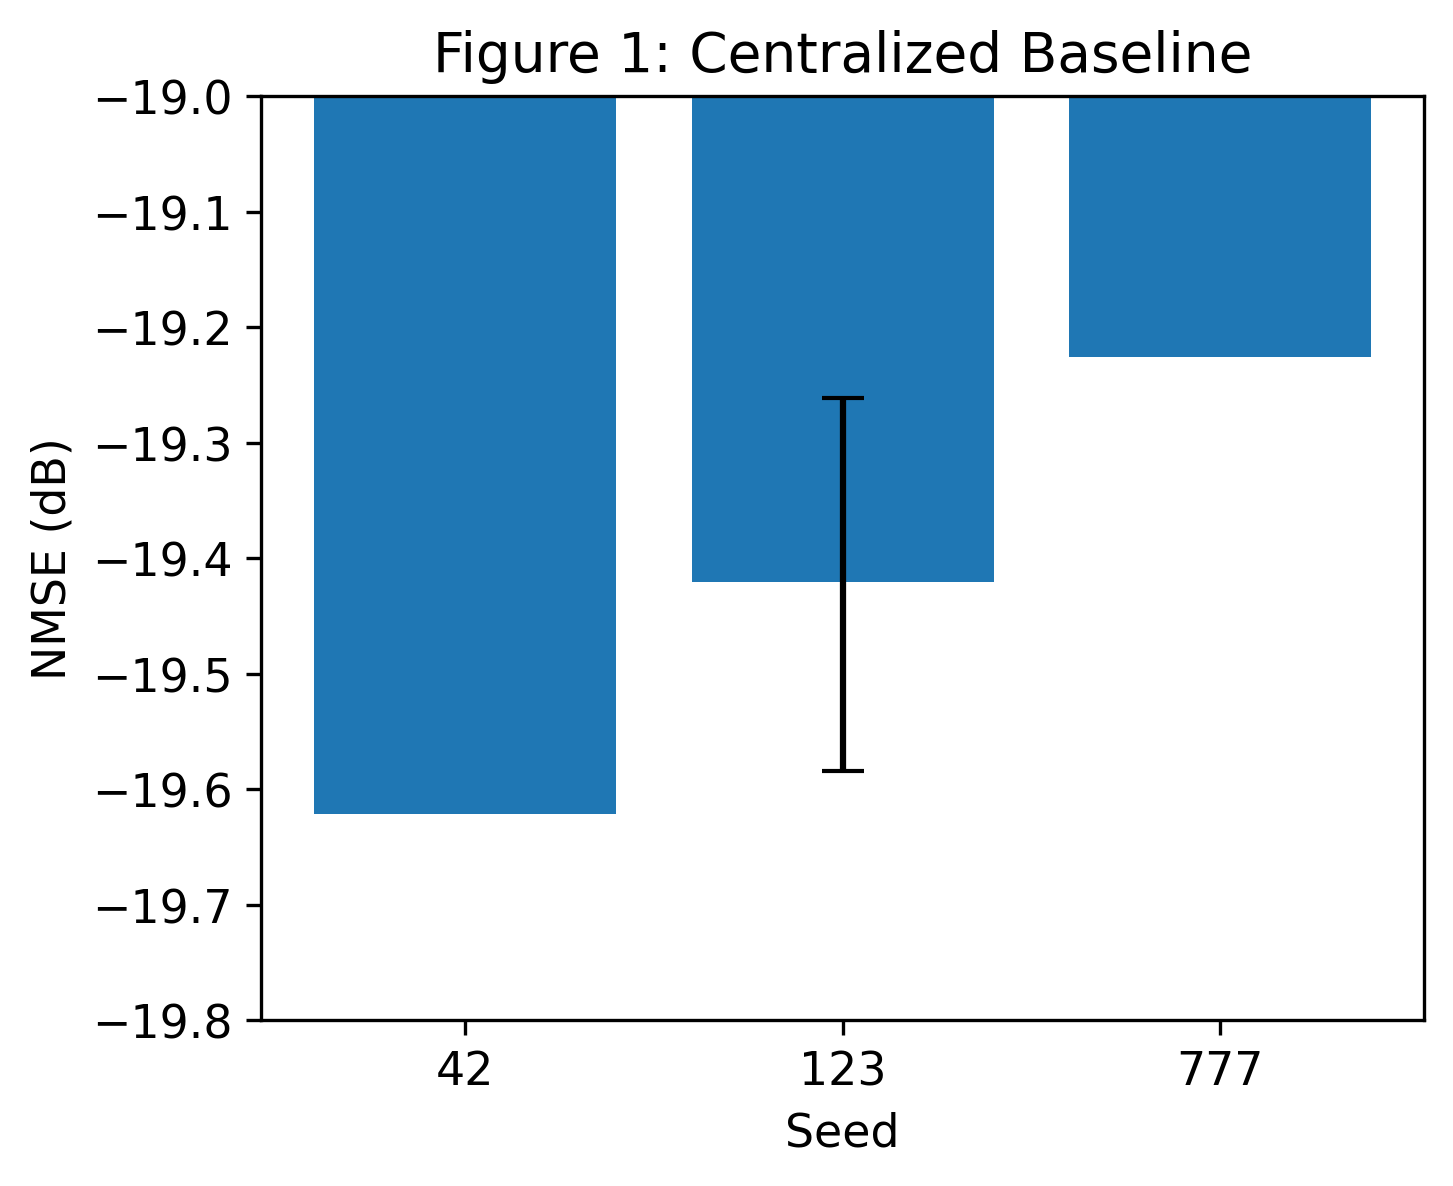
\includegraphics[width=0.75\columnwidth]{figures/figure1_centralized_baseline.png}
\caption{Baseline reproducibility with centralized setup for seeds (objective: stability of CL baseline).}
\label{fig:f1}
\end{figure}


\subsection{Convergence and Hyperparameter Effects}
\textbf{Purpose:} The objective of the experiment is to study the effects of global rounds and epochs (number of local iterations) on the quality of estimates.

\textbf{Observation:} NMSE improves with increase in both rounds and epochs for IID distributions. When transitioning from low to high budget for few rounds, there are significant increases in accuracy.

\textbf{Interpretation:} This is because it represents the typical behavior of FL optimization where each iteration of communications reduces the bias significantly, while each subsequent iteration optimizes the network. Increased epoch sizes help in better fitting locally, although there might be issues like drifting in case of heterogeneous data sets.

\textbf{Implication:} Knee point selection should be done for the operating point.

\begin{figure}[htbp]
\centering
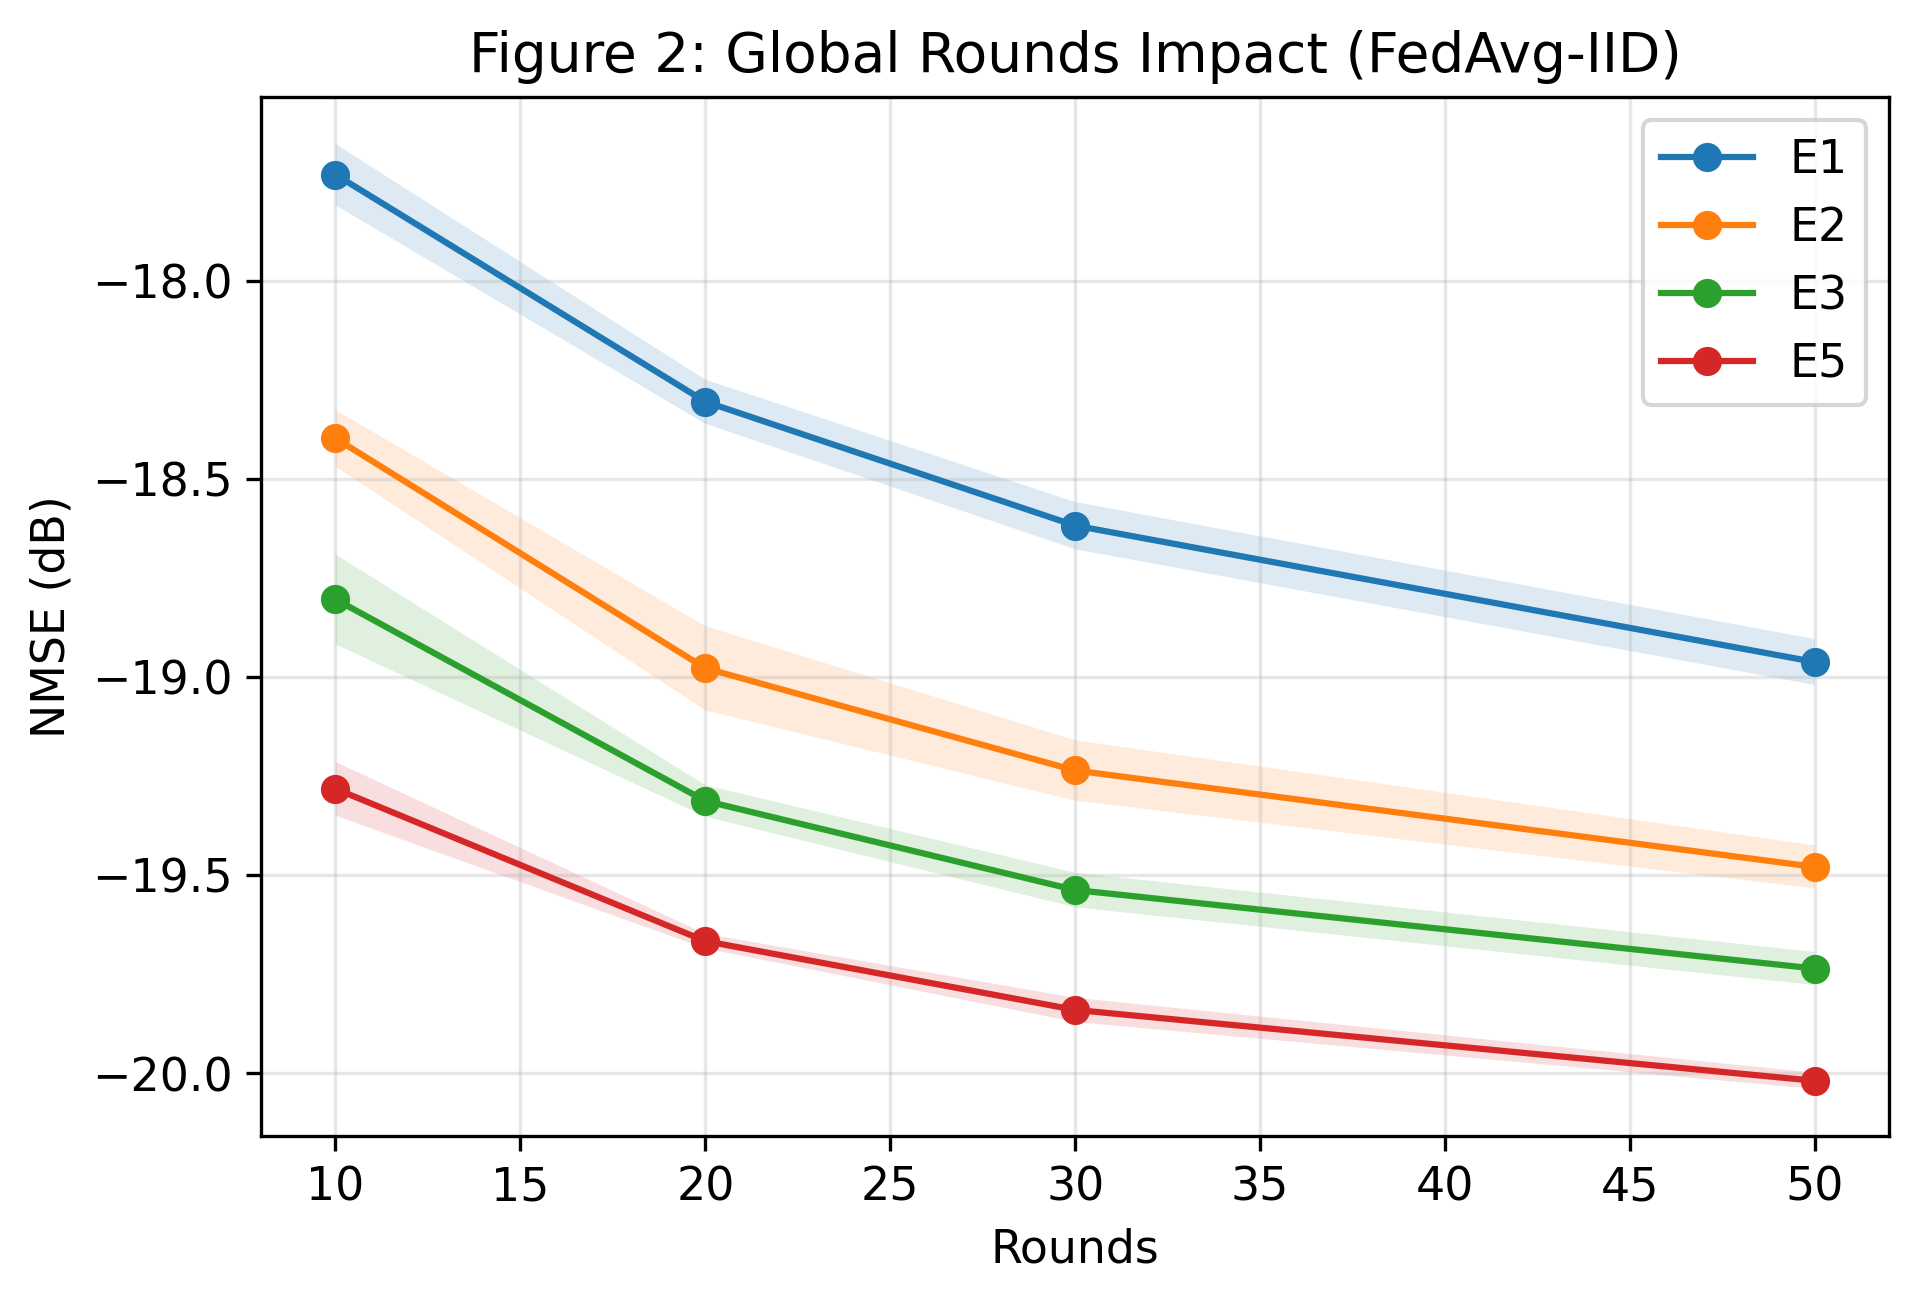
\includegraphics[width=0.65\columnwidth]{figures/figure2_rounds_impact_fedavg_iid.png}
\caption{Effect of FedAvg-IID round numbers: convergence rate and diminishing returns.}
\label{fig:f2}
\end{figure}

\begin{figure}[htbp]
\centering
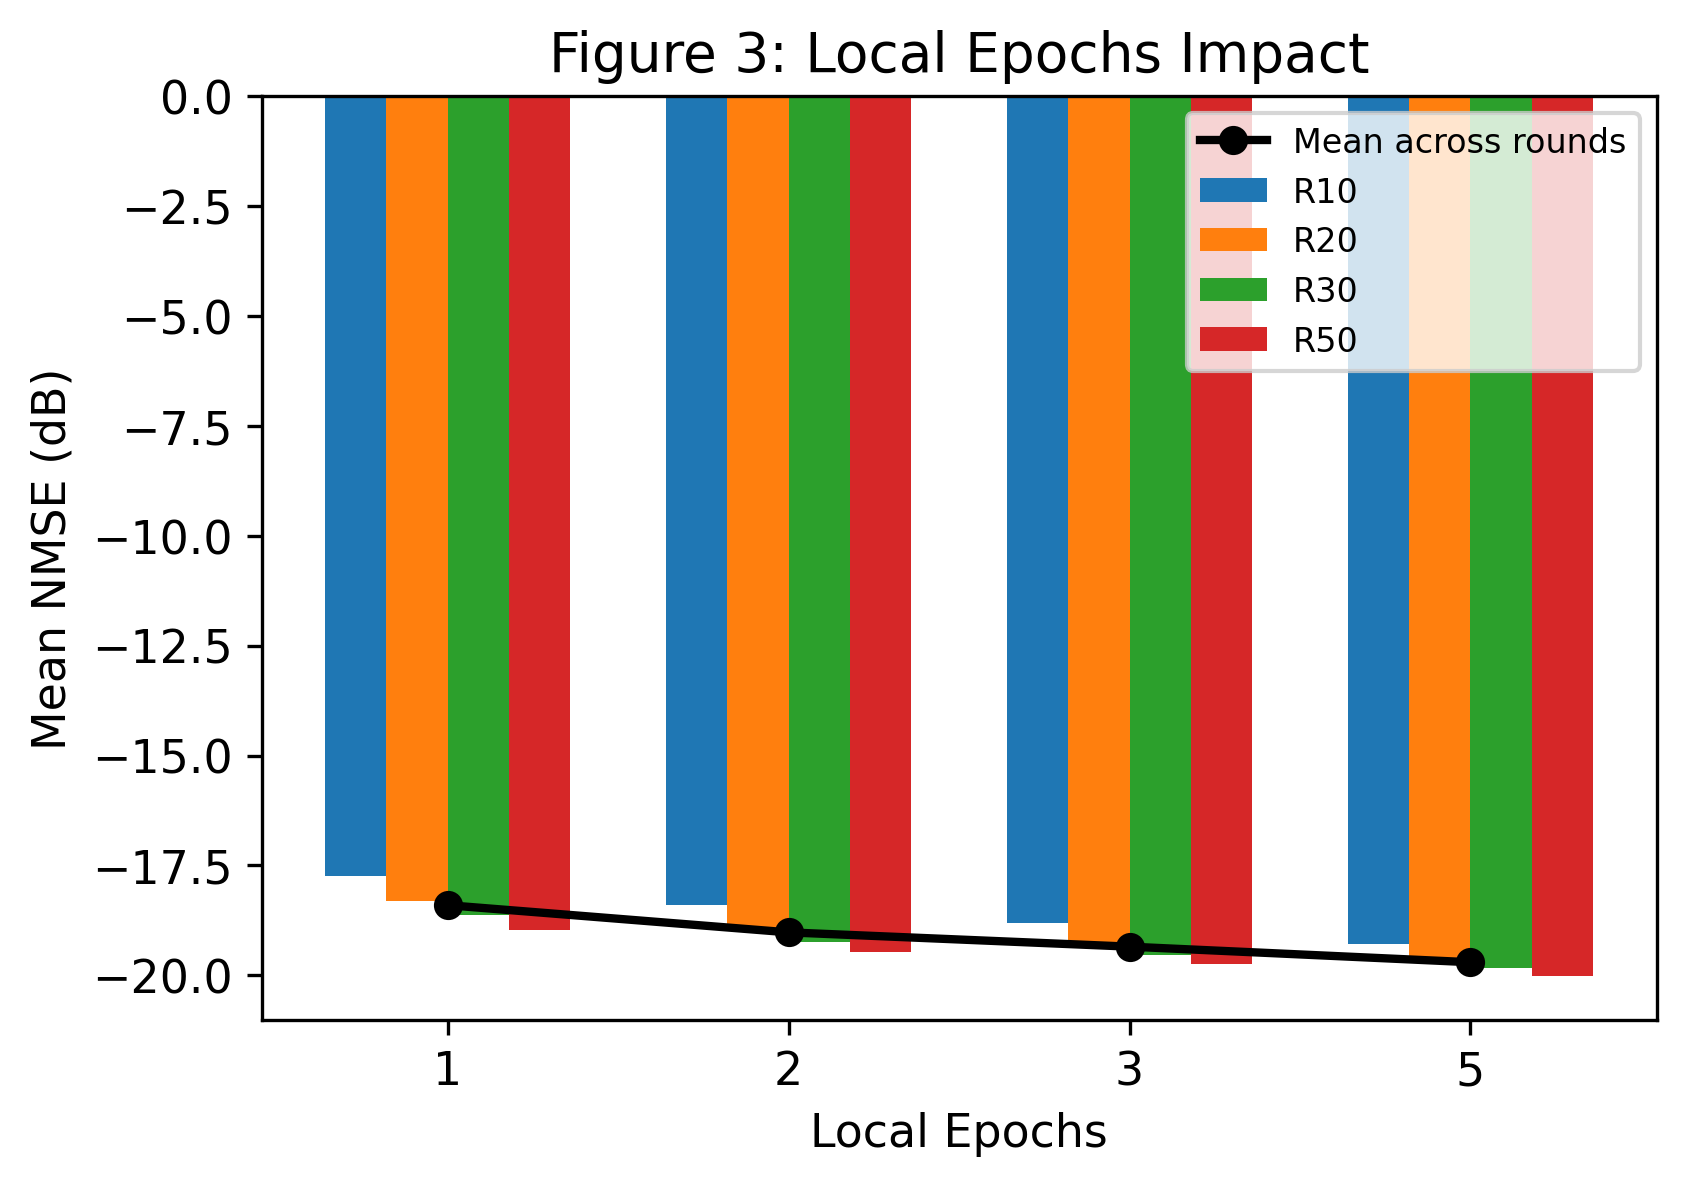
\includegraphics[width=0.65\columnwidth]{figures/figure3_local_epochs_impact.png}
\caption{Effect of number of local epochs: local computations vs global convergence performance.}
\label{fig:f3}
\end{figure}

\subsection{Convergence Dynamics}
\textbf{Purpose:} To establish trajectory information at the round level on stability and learning dynamics, rather than only end-point information.

\textbf{Observation:} Trajectories following the IID principle have smoother paths and achieve smaller NMSE values than those following the Non-IID principle.

\textbf{Interpretation:} The graph of convergence illustrates that heterogeneity is an intermediary issue and not simply an end-issue since it impacts the optimization procedure.

\textbf{Implication:} The algorithms used in Non-IID Learning should not depend solely on NMSE but instead on trajectory stability

\begin{figure}[htbp]
\centering
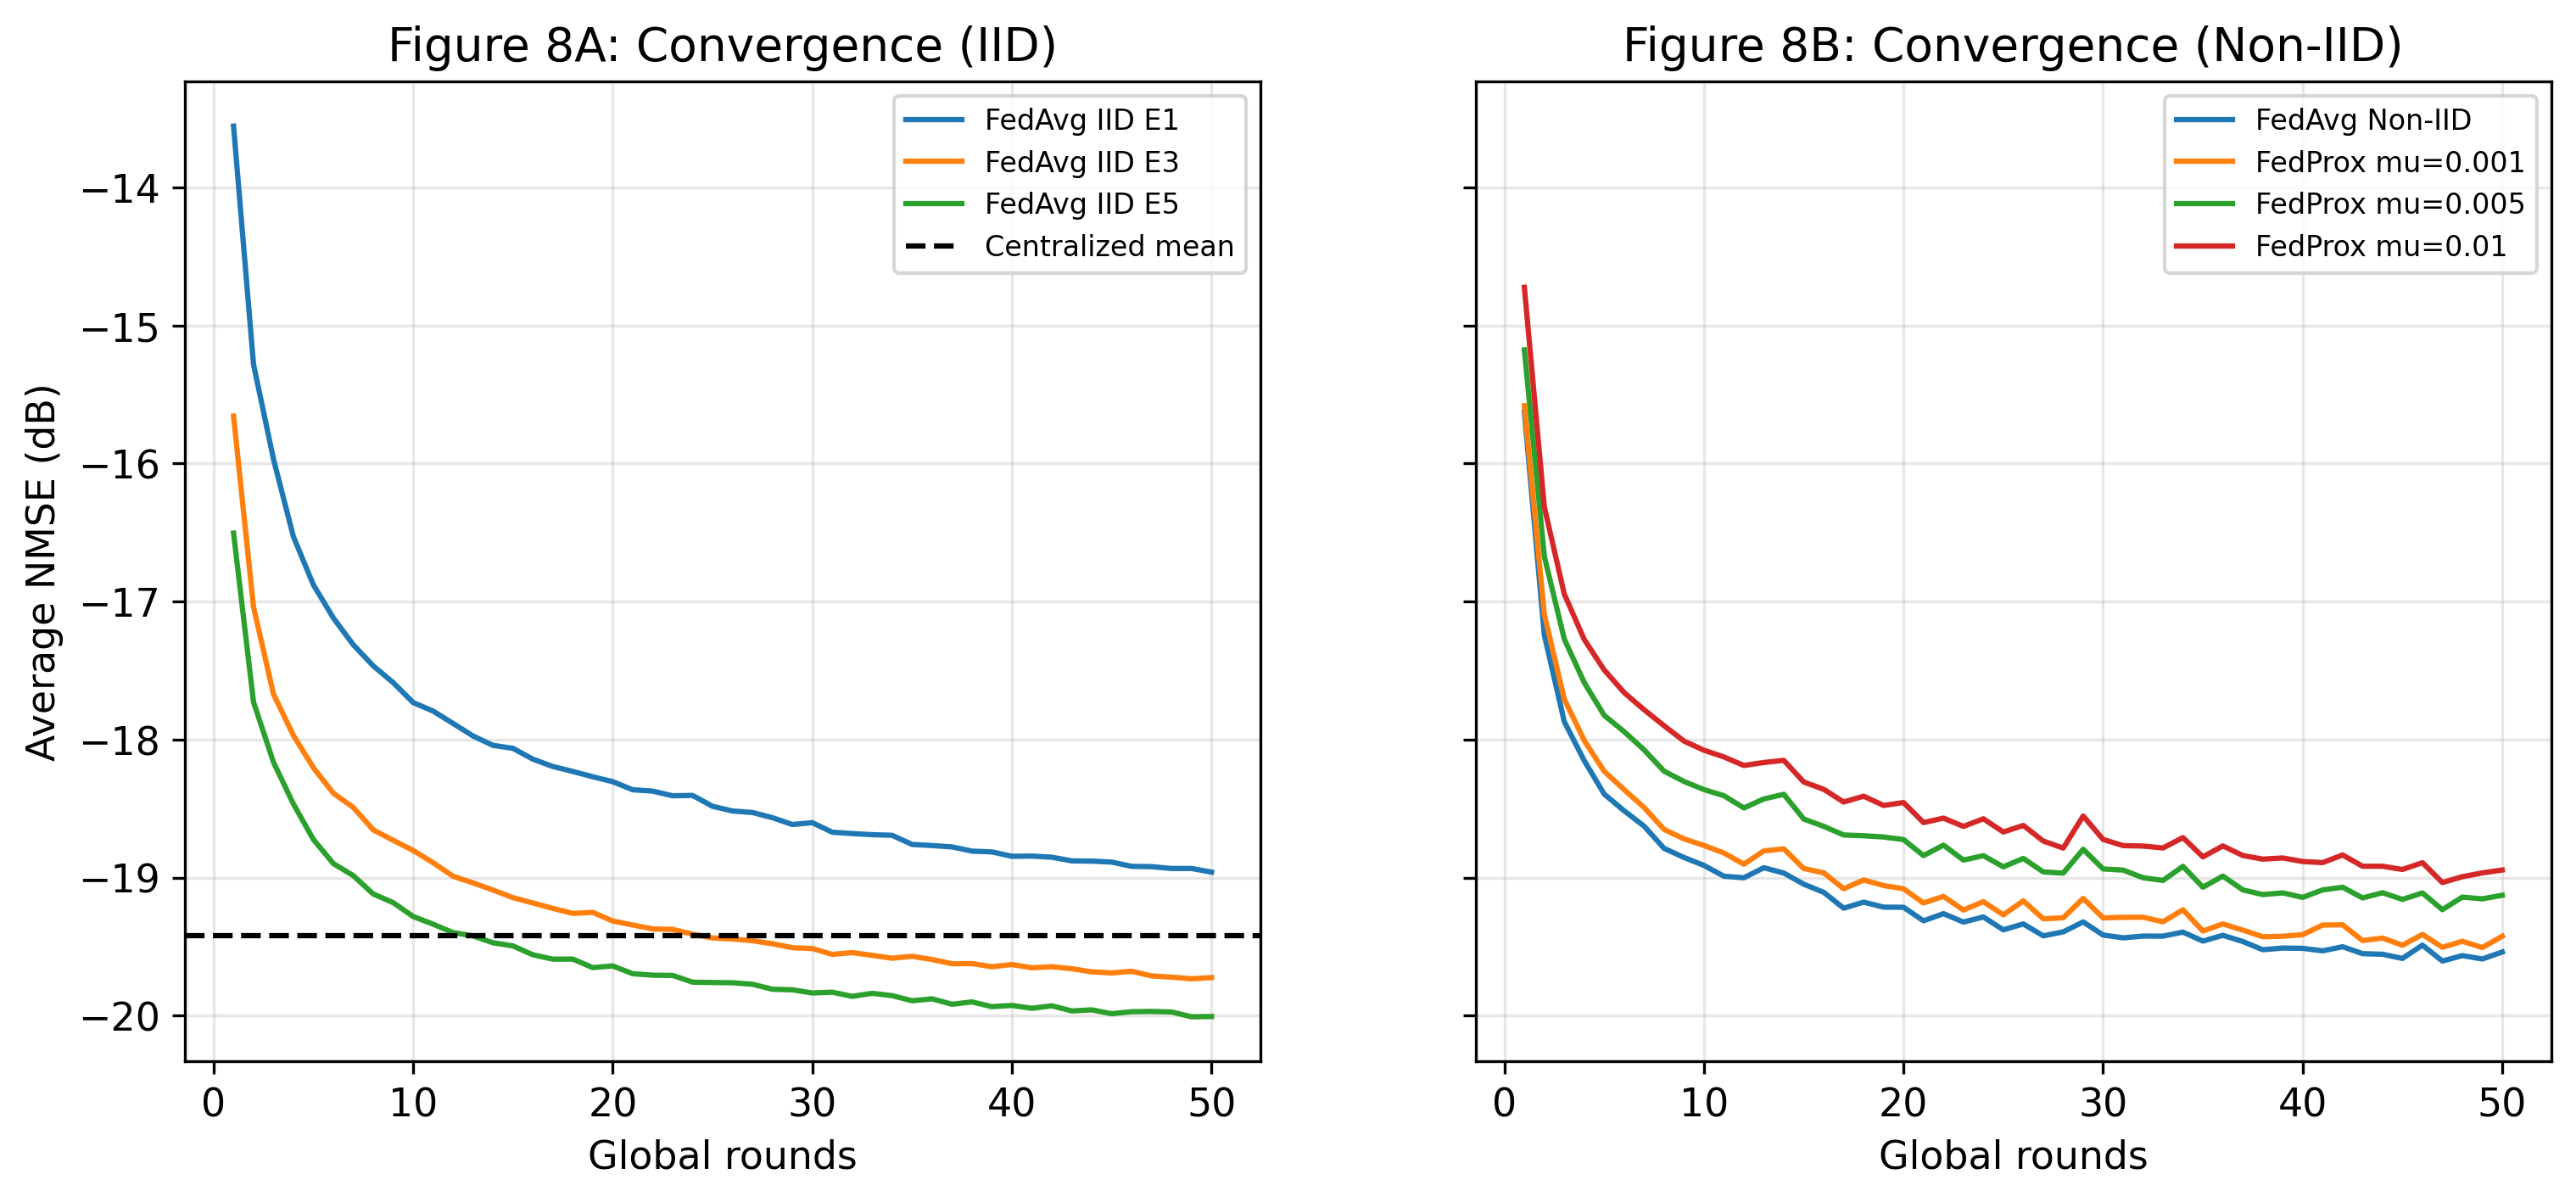
\includegraphics[width=0.75\columnwidth]{figures/figure8_convergence_curves.png}
\caption{Convergence trajectories for selected protocols .}
\label{fig:f8}
\end{figure}

\subsection{IID vs Non-IID and Algorithm Behavior}
\textbf{Purpose:} Cost incurred by changing distribution of the IID distribution and understand FedProx behavior relative to FedAvg.

\textbf{Observation:} Changing distributions is more expensive in the case of non-IID than IID distribution (higher NMSE value). In the comparison of FedAvg-IID vs. FedAvg-Non-IID, average difference is found to be 0.2707 dB. There exists statistical significance between them (Welch $p=0.0289$). Comparing the performance of FedAvg-Non-IID and FedProx-Non-IID gives the average difference to be 0.2800 dB (Welch $p=0.0044$).

\textbf{Interpretation:} Effect of non-IID can be measured statistically. FedProx doesn’t give superior performance regarding mean NMSE, but stability and gains from specific regime are its strengths.

\textbf{Best/mean/worst interpretation:} Larger variation shows more dependency on parameters/seeds, whereas smaller variation implies stability. Variation band ranges are larger for non-IID regime.

\begin{figure}[htbp]
\centering
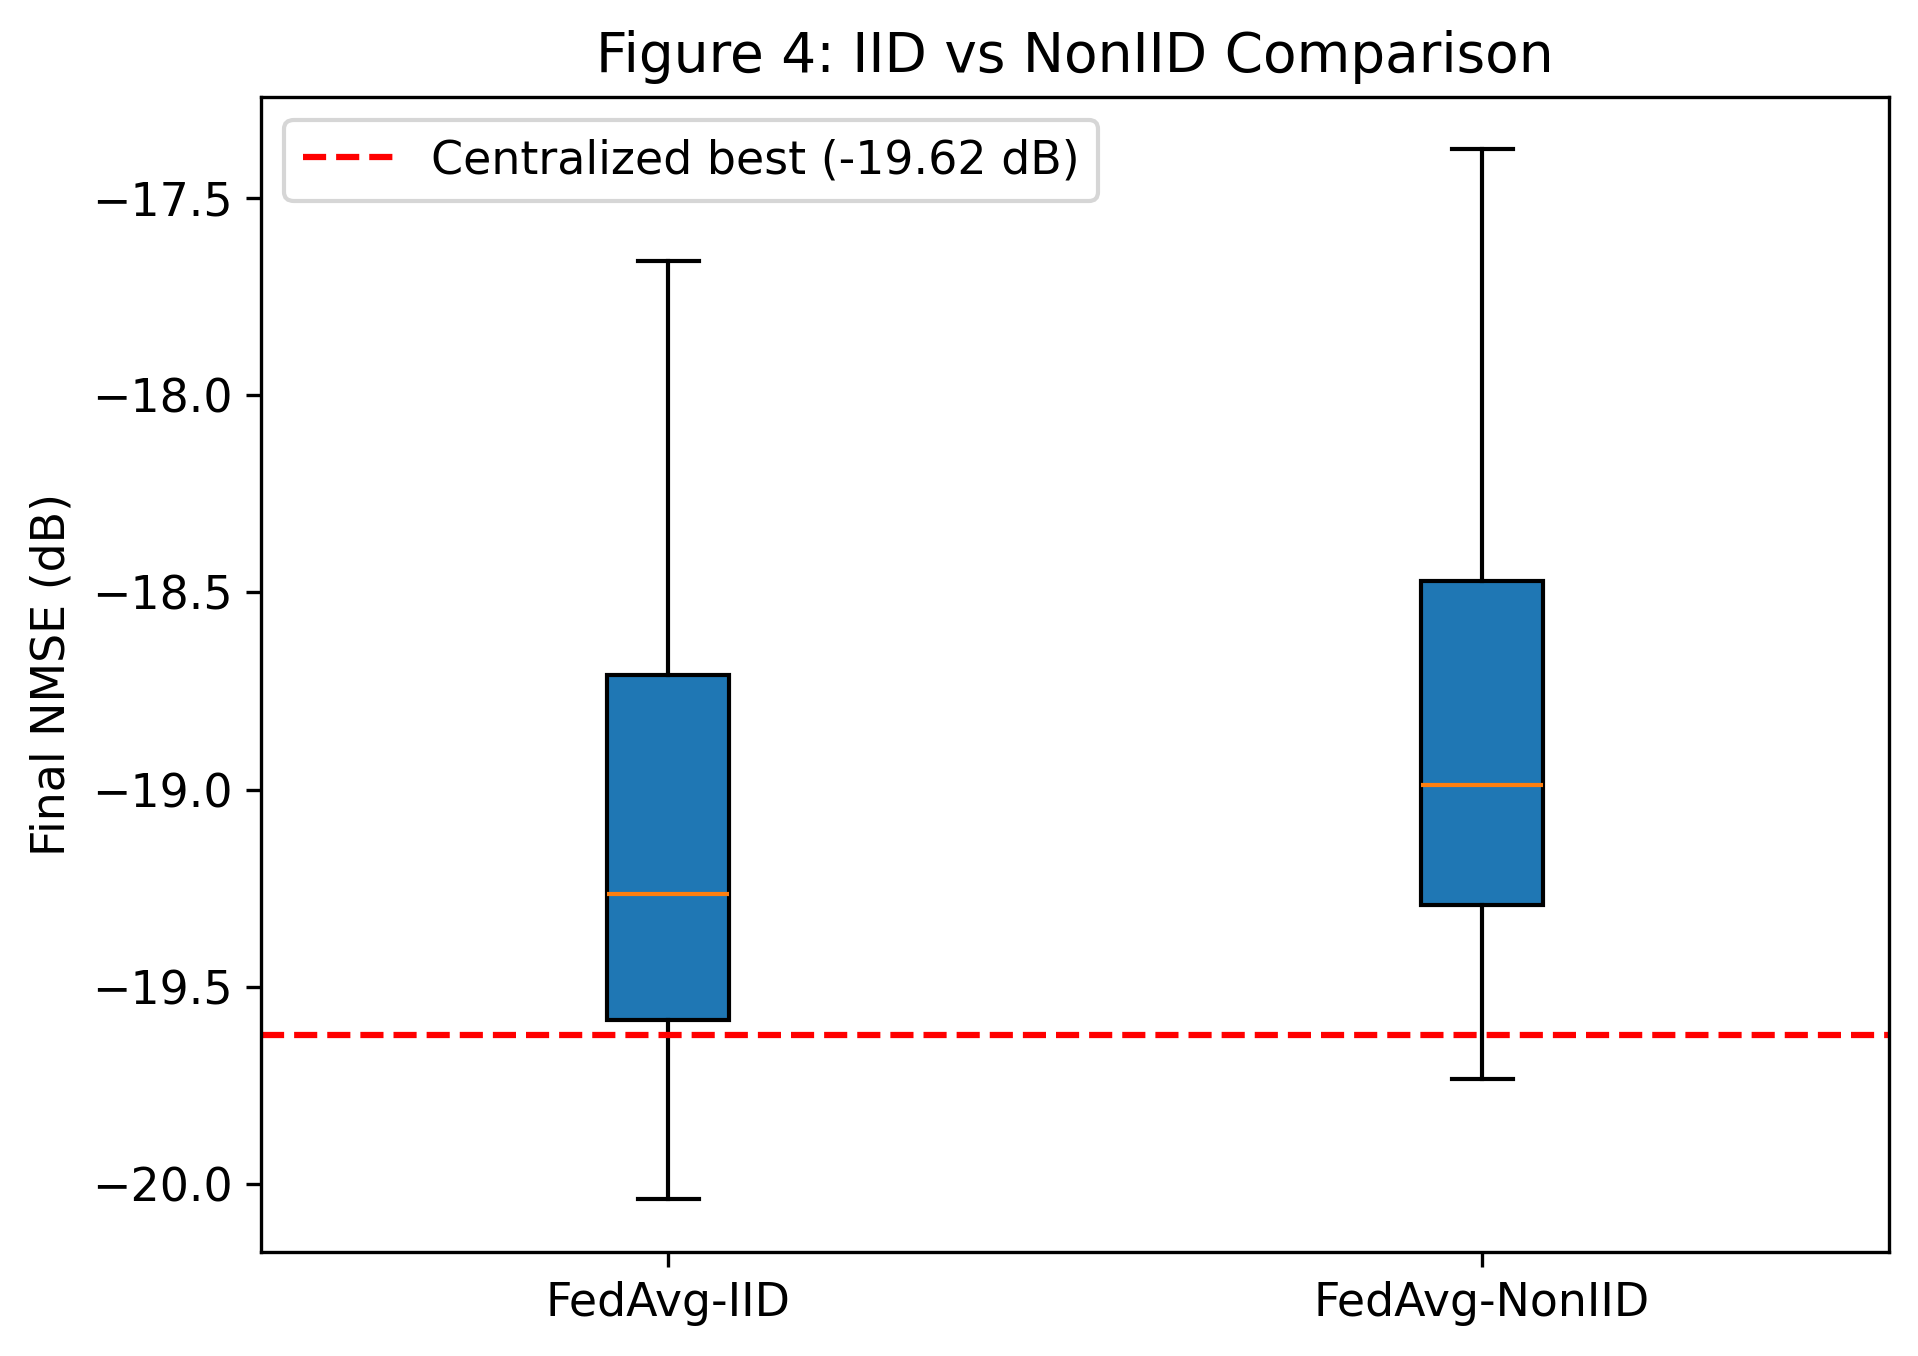
\includegraphics[width=0.75\columnwidth]{figures/figure4_iid_vs_noniid.png}
\caption{Comparison of IID and Non-IID distributions (objective: visualization of heterogeneity penalty).}

\label{fig:f4}
\end{figure}


\begin{figure}[htbp]
\centering
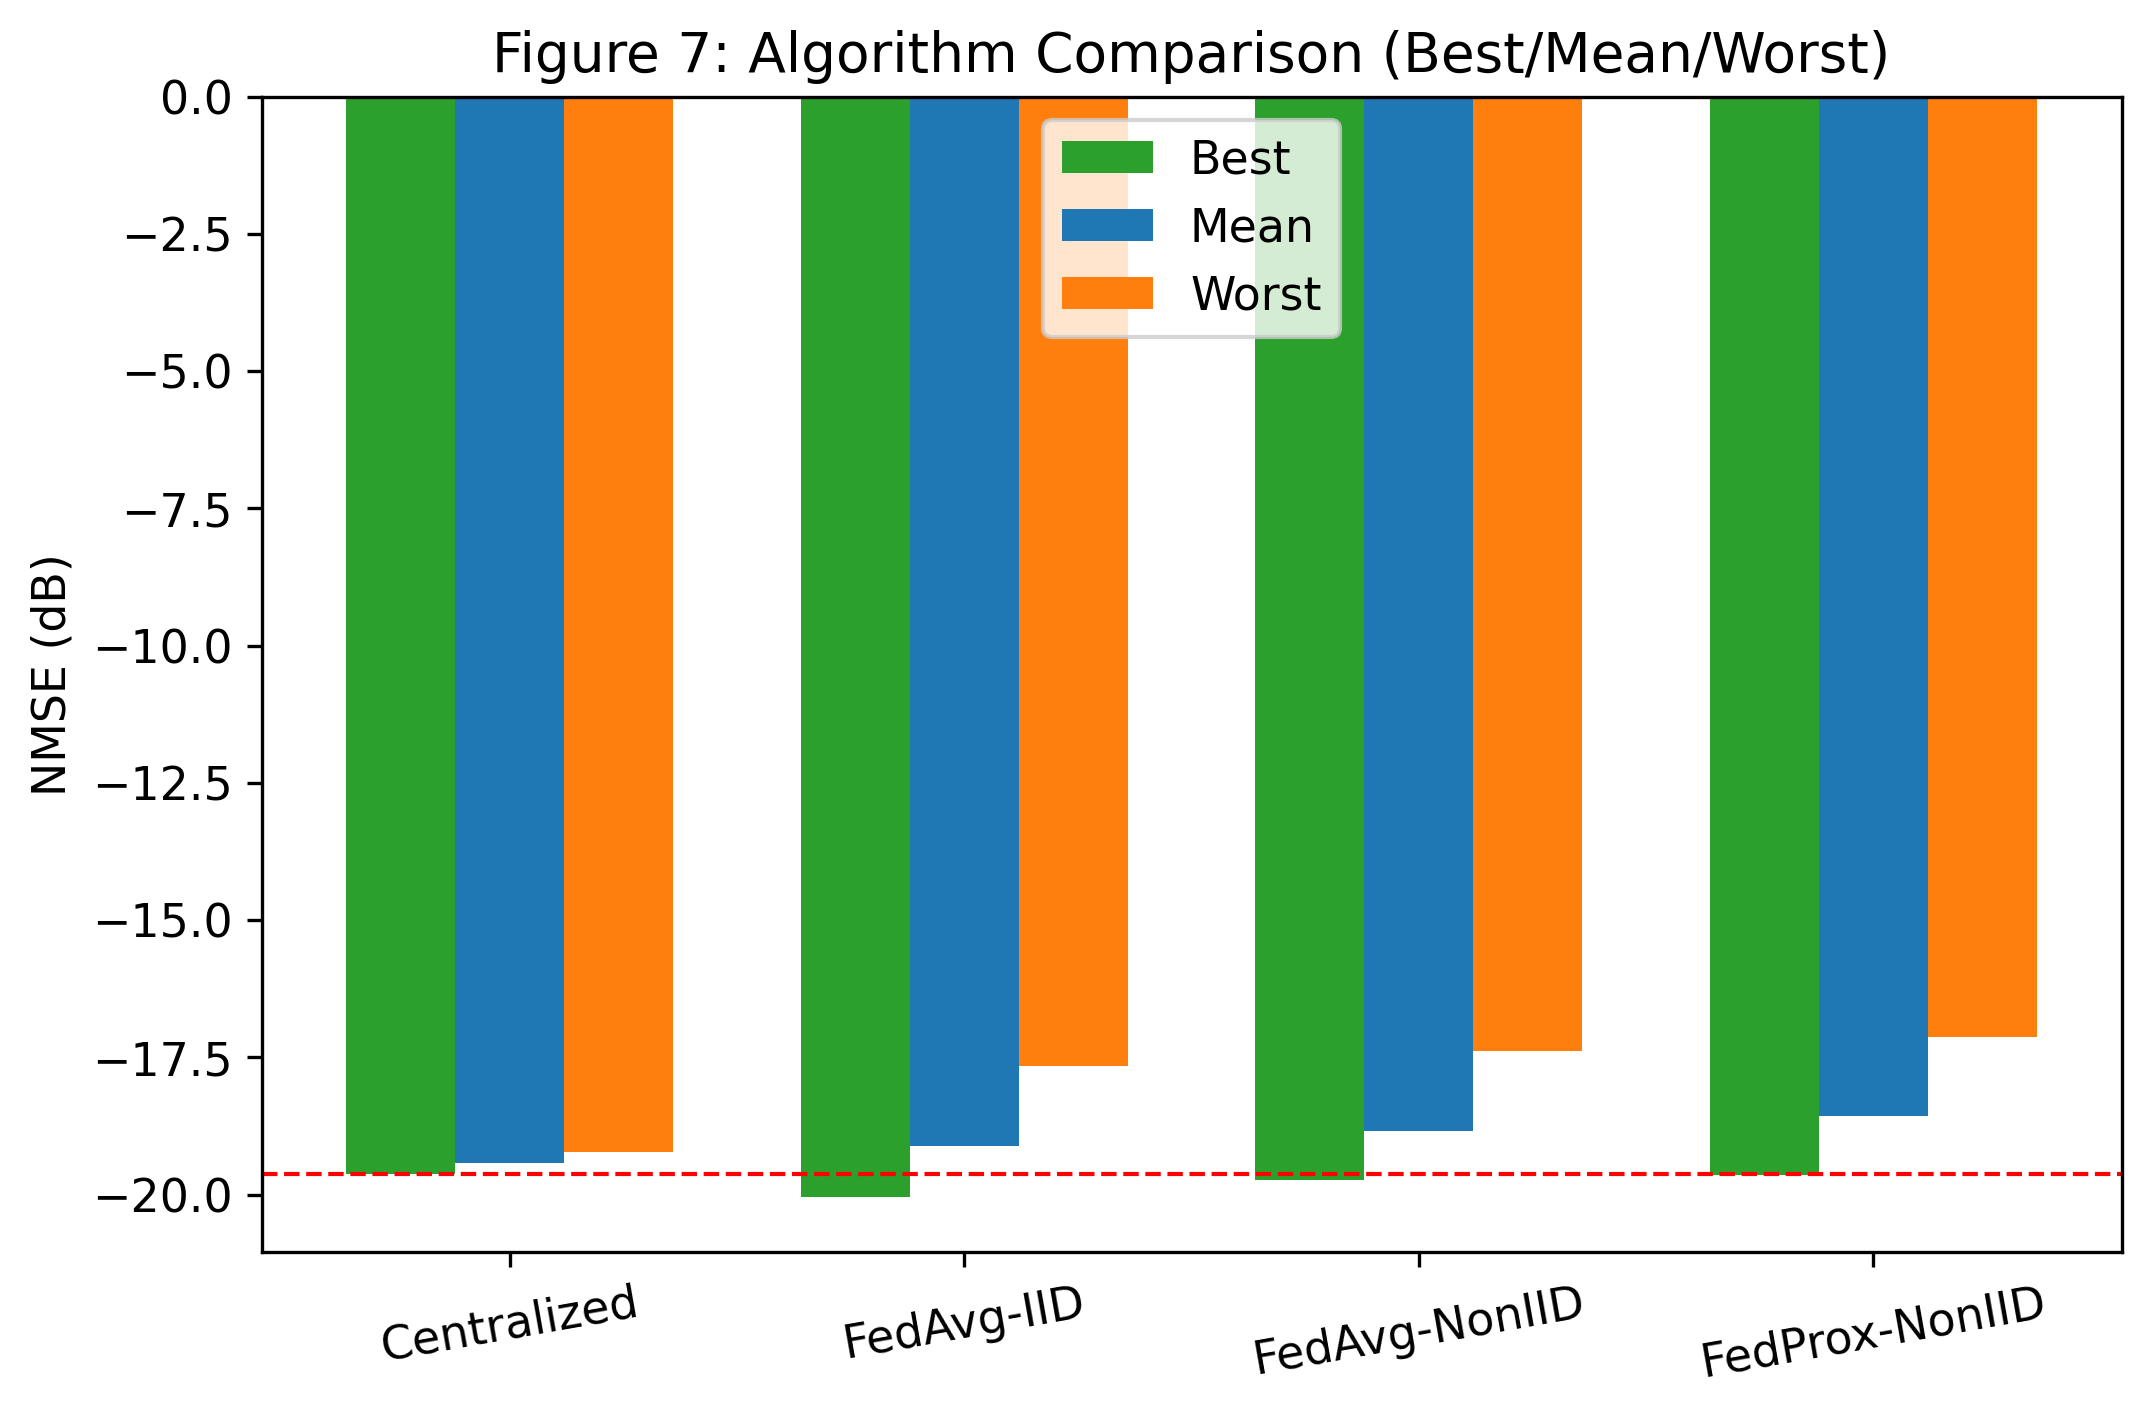
\includegraphics[width=0.75\columnwidth]{figures/figure7_algorithm_summary.png}
\caption{Best/Worst/Mean statistics (objective:interpretability of robustness).}
\label{fig:f7}
\end{figure}

\textbf{Implication:} For obtaining robust results, variability and confidence bands have to be considered alongside the means.

\subsection{Cross-Architecture Consistency (ResUNet Add-on)}
\textbf{Purpose:} check the sensitivity of heterogeneity findings to the model type

\begin{table}[htbp]
\caption{ResUNet Add-on Summary (5 Seeds/Setting)}
\label{tab:resunet}
\centering
\begin{tabular}{lcccc}
\toprule
Setting & Runs & Mean (dB) & Std (dB) & Best (dB) \\
\midrule
Centralized & 5 & -22.1210 & 0.3934 & -22.5281 \\
FedAvg-IID & 5 & -22.8969 & 0.1327 & -23.0406 \\
FedAvg-Non-IID & 5 & -21.1819 & 0.3369 & -21.6237 \\
FedProx-Non-IID & 5 & -20.4661 & 0.1393 & -20.6357 \\
\bottomrule
\end{tabular}
\end{table}

\begin{figure}[htbp]
\centering
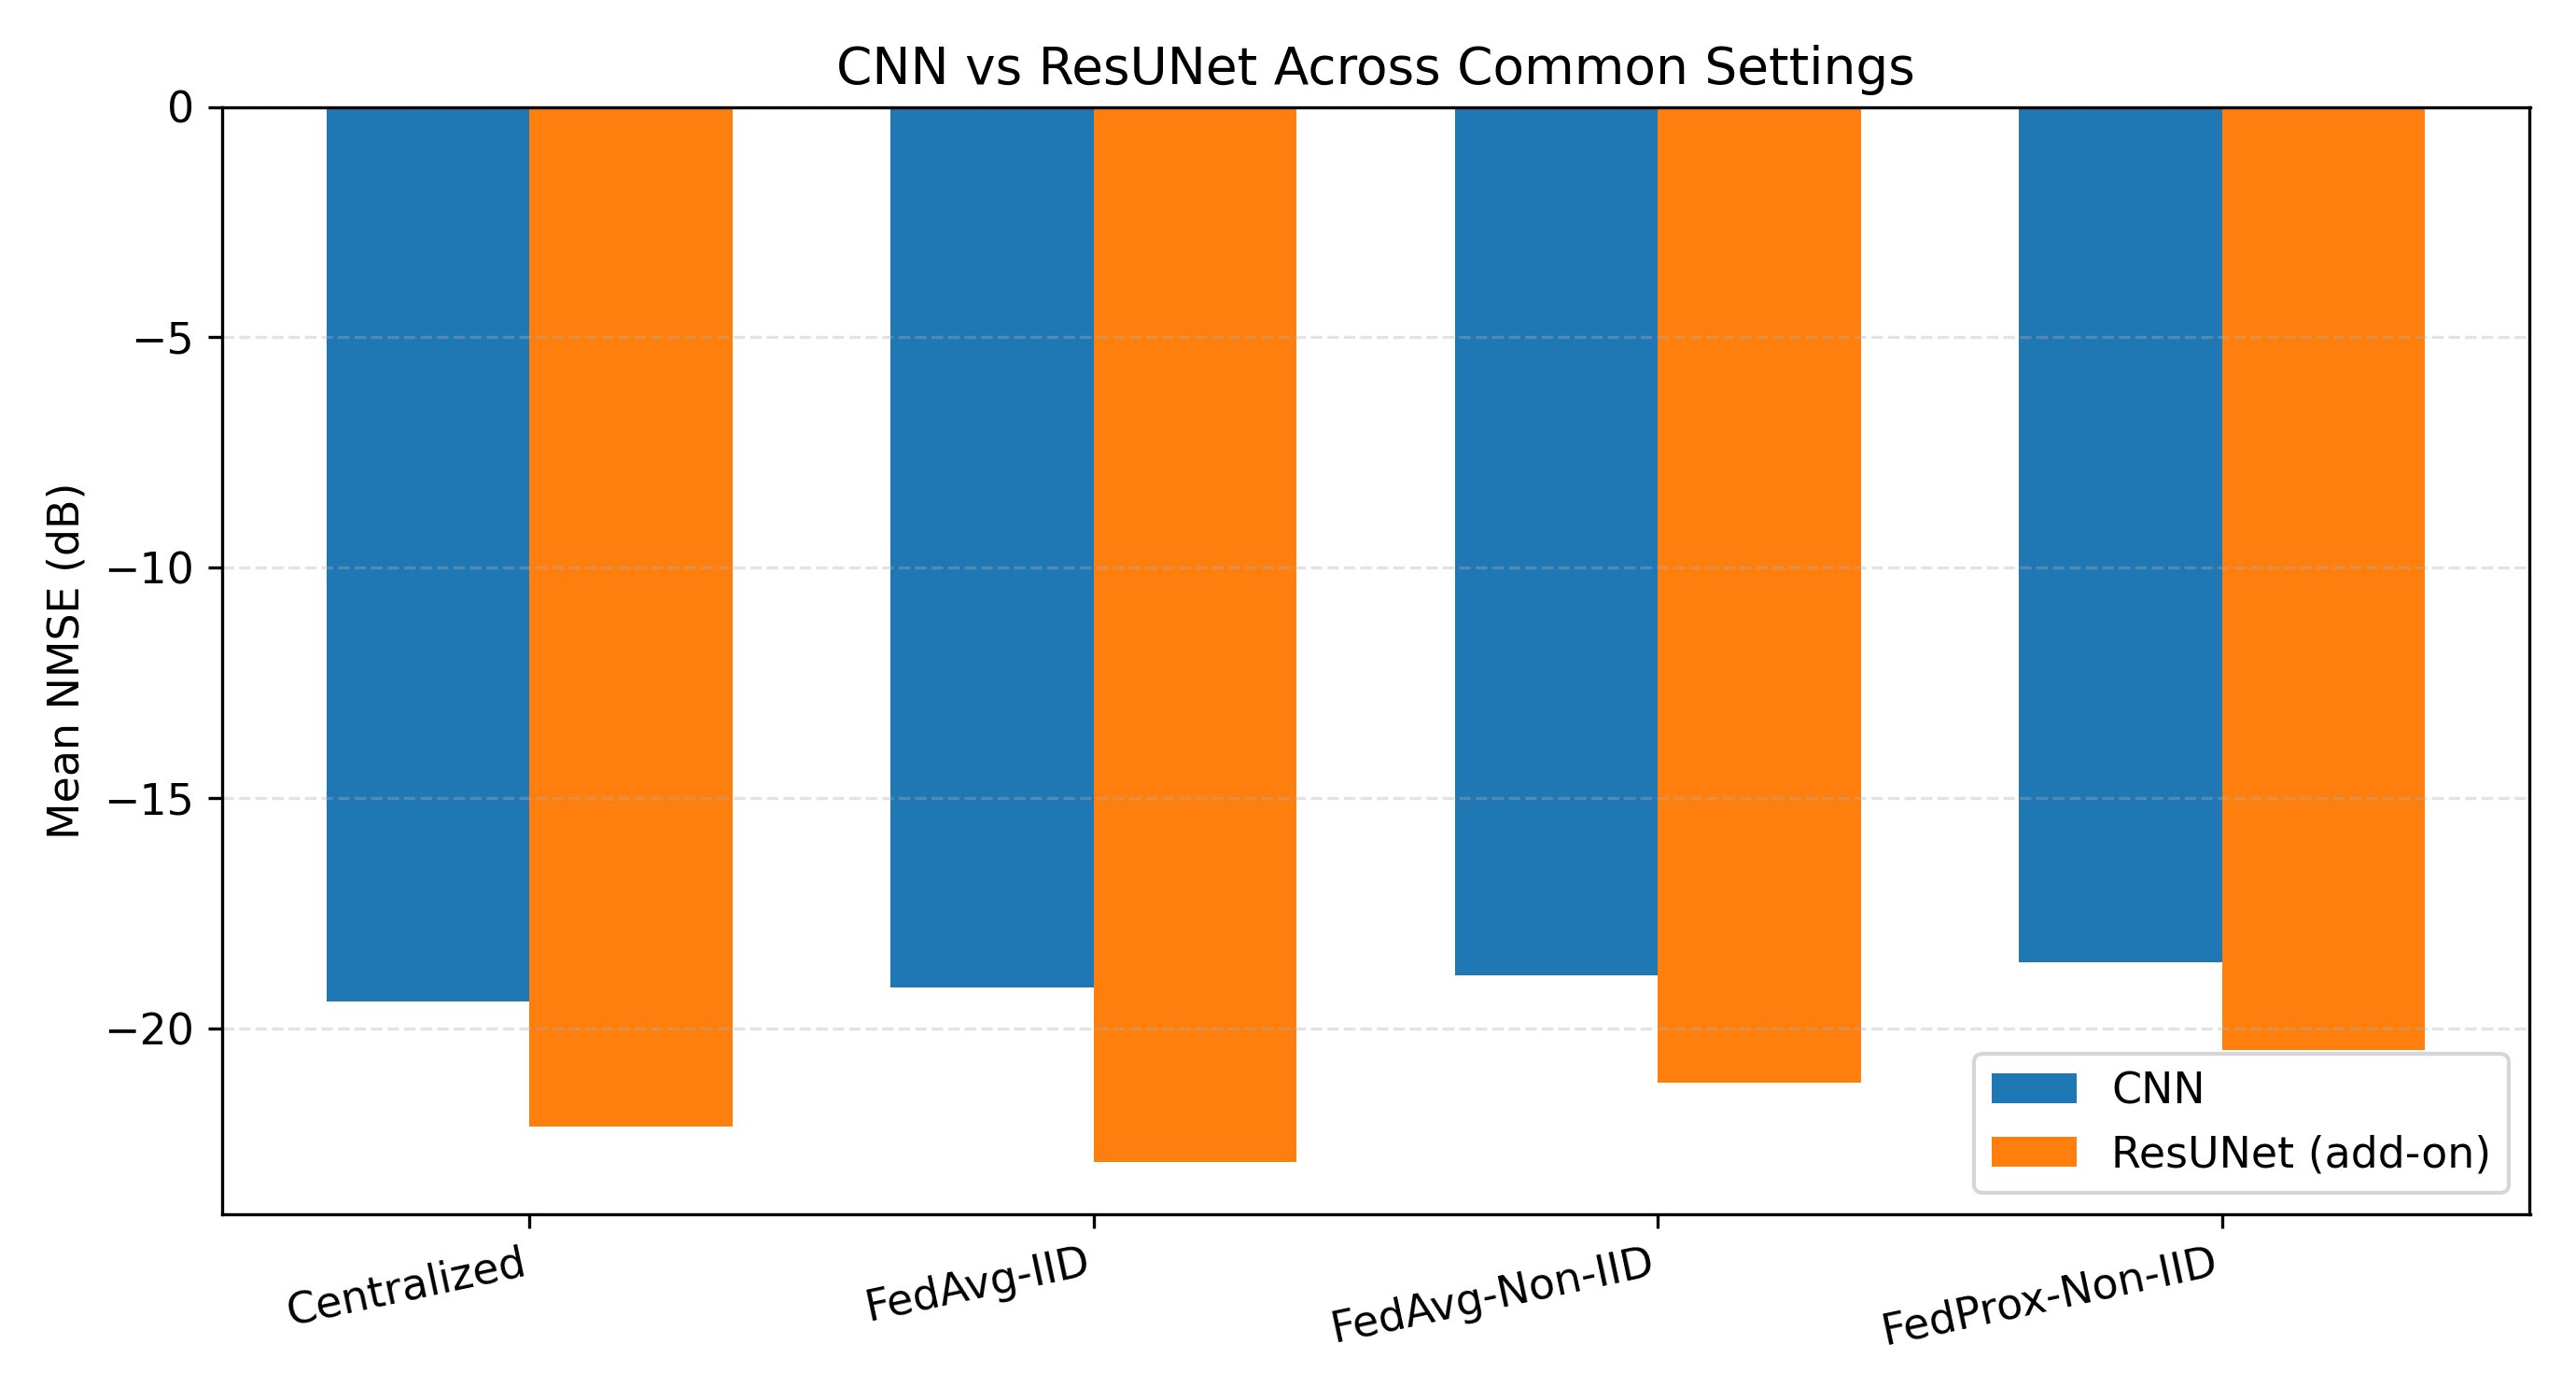
\includegraphics[width=0.75\columnwidth]{figures/resunet_addon_cnn_vs_resunet.png}
\caption{CNN vs ResUNet under aligned settings (purpose: trend portability across architectures).}
\label{fig:cross}
\end{figure}

\textbf{Observation:} ResUNet reproduces core trend directions: FedAvg-IID is strongest federated setting, and Non-IID causes substantial degradation. Specifically, FedAvg-Non-IID degrades by +1.7150 dB vs FedAvg-IID.

\textbf{Interpretation:} heterogeneity penalty persists across shallow and encoder-decoder architectures, indicating a data-distribution effect rather than a single-model artifact.

\textbf{Implication:} mitigation strategies for Non-IID should be treated as pipeline-level priorities, not architecture-only fixes.

\subsection{Classical Baseline and Communication Analysis}
\textbf{Purpose:} place deep models relative to classical LS and quantify systems cost.

\begin{table}[htbp]
\caption{Classical Baseline Comparison (10 dB SNR)}
\label{tab:classical}
\centering
\begin{tabular}{p{0.22\linewidth}p{0.14\linewidth}p{0.54\linewidth}}
\toprule
Method & NMSE (dB) & Note \\
\midrule
LS & -10.00 & $\hat{H}=\tilde{H}$ (no processing) \\
Scalar LMMSE & -10.41 & Train-calibrated scalar shrinkage \\
Full-Cov MMSE & -28.55 & Wiener filter with sample $R_{HH}$ \\
\midrule
CNN (CL mean) & -19.42 & 19,778 params; no $R_{HH}$ needed \\
ResUNet (CL mean) & -22.12 & 763,234 params; no $R_{HH}$ needed \\
\bottomrule
\end{tabular}
\end{table}

\textbf{Observation:} The full-covariance MMSE estimator achieves -28.55 dB at 10 dB SNR, substantially outperforming both the scalar LMMSE (-10.41 dB) and the deep learning models. However, the full-covariance MMSE requires explicit knowledge of the channel covariance matrix $R_{HH}$, which must be estimated from training data and inverted ($O(d^3)$ complexity for $d=8192$). However, the CNN and ResUNet learn their estimation scheme through the training data itself without computing the covariances.

\textbf{Interpretation:} These two DL algorithms present a practical approach in that they surpass the single-valued LMMSE algorithm significantly (+9.01 dB for CNN, +11.70 dB for ResUNet) but without the computational burden of calculating the covariances and inverting the matrices which is the case with the full MMSE algorithm.
Especially federated learning scenarios because in such cases, each device will be required to compute their own $R_{HH}$locally and invert it.

\textbf{Implication:} Essentially, the FL approach has been updated so that federated deep learning can provide the optimal solution regarding accuracy vs complexity in federated learning since federated learning provides better performance than the linear approaches and does not need channel statistics while carrying out operations in devices with low computation power.

Uplink Payload Size for the communication model (FP32)
\begin{equation}
\mathcal{C}_{\text{round}}\approx 4P,\qquad
\mathcal{C}_{\text{total}}\approx 4PKR.
\end{equation}
For $K{=}5, R{=}50$: CNN (19,778 params) requires Upto 18.86 MB total uplink payload, while ResUNet (763,234 params) requires Upto 727.88 MB.

\textbf{Interpretation:} Communication overhead is linearly dependent on both the size of the model and the iterations in federated learning. The architecture that improves NMSE the most may also be the least communication-efficient.

\textbf{Computational Complexity (FLOPs) Analysis:} Apart from the communication payload, the other component that adds to the computational complexity of federated learning is the computation done by the client devices for both the forward and backward passes at the client-side.
\begin{itemize}
    \item \textbf{CNN:} The simplicity of the architecture and smaller receptive field of this network (total of 19,778 parameters) make it have a computational cost of roughly \textasciitilde 160 MegaFLOPs (MFLOPs). Thus, it is ideal for resource-constrained clients. 
    \item \textbf{ResUNet:} With a deeper network architecture (763,234 parameters), the
computation for a single inference involves roughly \textasciitilde 2.5 GigaFLOPs (GFLOPs).
\end{itemize}
Though ResUNet offers better NMSE results, its computational complexity is an order of magnitude greater compared to that of the CNN, which makes the consumption of energy much greater on clients with limited power supply.

\textbf{Implication:} Communication-conscious selection of models becomes vital for implementing FL practically.



\begin{table}[htbp]
\caption{Communication Cost Snapshot (CNN)}
\label{tab:comm}
\centering
\begin{tabular}{lccc}
\toprule
Configuration & Comm. Events & NMSE (dB) & Efficiency \\
\midrule
FedAvg-IID (R10,E1) & 50 & -17.7319 & Low \\
FedAvg-IID (R30,E3) & 150 & -19.5375 & Medium \\
FedAvg-IID (R50,E5) & 250 & -20.0190 & High \\
Centralized (20 ep) & 0 & -19.4227 & -- \\
\bottomrule
\end{tabular}
\end{table}


\section{Discussion}

\textbf{Advantages of ResUNet.} Multi-scale Encoder-Decoders and Skip Connections facilitate the preservation of the structure and elimination of noise using ResUNet. ResUNet seems promising in image reconstruction, particularly when shallow CNNs are inadequate for reconstruction.

\textbf{Drawbacks of Non-IID Assumption.} Clients use distinct loss functions owing to the non-IID assumption. This would lead to conflicting gradients during gradient aggregation.

\textbf{Inconsistency in FedProx.}The ($\mu$) regularization  used in FedProx stabilizes the model but prevents any local updates. Its functionality relies on heterogeneity, number of epochs, and model capacity. Hence, accuracy and stability can’t coexist simultaneously.

\textbf{Instability in FedProx.} The issue of FedProx instability is similar to that of hyperparameter and regime mismatching. Three pieces of evidence support this:
\begin{itemize}
    \item \textbf{$\mu$ sensitivity:} ablation over $\mu\in\{0.001,0.005,0.01\}$ shows best mean performance at $\mu=0.001$ and a 0.423 dB sensitivity span, indicating over-regularization at larger $\mu$.
    \item \textbf{Local epoch interaction:} local epochs show a larger 0.9731 dB sensitivity span with best value at $E=5$, suggesting that too few local epochs can make proximal regularization dominate before sufficient local fitting occurs.
    \item \textbf{Statistical evidence:} FedAvg-Non-IID vs FedProx-Non-IID mean gap is significant (Welch $p=0.0044$), confirming the degradation is systematic in the tested regime.
\end{itemize}



Taken together, the likely cause is a combination of higher $\mu$ settings and limited local adaptation under heterogeneity, not the absence of any potential FedProx benefit.



\section{Conclusion}
In this paper, we have developed a federated learning architecture for massive MIMO channel estimation. This paper compares the performance of the FedAvg and FedProx algorithms to traditional channel estimators (LS, LMMSE, and MMSE). The results obtained from our experiment show that FL is a promising solution to channel estimation. In particular, the optimal settings of FedAvg-IID outperform the centralized approaches by a small margin in NMSE, demonstrating that FL training preserves model performance.


The introduction of a non-IID distribution to clients' datasets causes a consistent heterogeneity overhead of around 0.3 dB and greater variability, but techniques such as FedProx can solve this problem. On the other hand, while
the full covariance-based MMSE approach sets a theoretical upper bound, deep learning models circumvent costly $O(d^3)$ matrix inversion through a better balance between accuracy and computational complexity.


Even if our results at the moment are convincing, our evaluations can only be made within the range of 10 dB SNR, while the MMSE baseline is based on a fully centralized and offline covariances knowledge. It would be worthwhile to conduct studies with multiple SNRs ranges (0–20 dB) and to study pilot-based distributed covariance estimation in the future to increase practicality. Another important task is to study personalization of Non-IID data and apply Differential Privacy in CSI feedbacks.

\bibliographystyle{splncs04}
\bibliography{main}



\end{document}
